% Created 2023-03-21 Tue 15:53
% Intended LaTeX compiler: pdflatex
\documentclass[11pt]{article}
\usepackage[utf8]{inputenc}
\usepackage[T1]{fontenc}
\usepackage{graphicx}
\usepackage{longtable}
\usepackage{wrapfig}
\usepackage{rotating}
\usepackage[normalem]{ulem}
\usepackage{amsmath}
\usepackage{amssymb}
\usepackage{capt-of}
\usepackage{hyperref}
\usepackage{tikz, pgfplots}
\usepackage{import}
\author{Lokesh Mohanty}
\date{\today}
\title{Neural Networks}
\hypersetup{
 pdfauthor={Lokesh Mohanty},
 pdftitle={Neural Networks},
 pdfkeywords={},
 pdfsubject={},
 pdfcreator={Emacs 29.0.60 (Org mode 9.7-pre)}, 
 pdflang={English}}
\begin{document}

\maketitle
\tableofcontents

\section{Introduction}
\label{sec:neural-networks}

If $h_{\theta}(x)$ is our hypothesis function, then
\begin{align*}
h_{\theta}(x) &= w_2^T\sigma_1 \left( w_1^T x \right)
\end{align*}
where $w_1, w_2$ are the parameter matrices for layer 1 and 2 and $\sigma_1$ is the activation function of layer 1. By definition $\sigma$ is an asymptotic function $\left(\text{i.e., }\sigma(x) = \begin{cases} 0, x \rightarrow -\infty  \\ 1, x \rightarrow \infty \end{cases} \right)$.

\begin{align*}
  x \in \mathbb{R}^d,& y \in \mathbb{R}^k \\
  w_1 \in \mathbb{R}^{d \times l},& w_2 \in \mathbb{R}^{l \times k}
\end{align*}
  $w^l_{jk} \rightarrow$ weight from $k^{th}$ neuron in $(l-1)^{th}$ layer to $j^{th}$ neuron in the $l^{th}$ layer \\

\paragraph{} In neural networks we just use a complex hypothesis function which can be a universal approximator. We can have a single or multiple layers of neurons which together forms the hypothesis function. This is also called a \textit{Multi-Layer Perceptron (MLP)}. If all the neurons are connected, it is called a \textit{Fully connected neural network}.

\section{Universal Approximation Theorem (UAT)}
Suppose $f(x): \mathbb{R}^d \rightarrow \mathbb{R}^k$

\begin{align*}
  h_{\theta}(x) &= w_2^T \sigma_1(w_1^Tx) \\
  w_1 \text{ and } &w_2 \text{ s.t. } |f(x) - h_{\theta}(x)| \leq \epsilon\\
  \epsilon > 0 &, \delta > 0
\end{align*}

\section{Error-back Propagation (Chain rule)}
\label{sec:error-back-prop}

We need to find the hypothesis function by training the parameters. This is done by empirical risk minimization. We use a method \textit{Error-back propagation} to train the parameters.\\

\underline{Activation Notations:}
\begin{itemize}
\item $a^l = \sigma \left( w^l a^{l-1} + b^l \right)$
\item $a^l_j =$ activation of $j^{th}$ neuron in $l^{th}$ layer
\item $a^l_j = \sigma \left( \sum_k w_{jk}^l a_k^{l-1} + b_j^l \right)$
\item $z^l \triangleq w^la^{l-1} + b^l$
\end{itemize}

\begin{align*}
  \frac{\partial \hat{R}}{\partial w^l_{jk}} &= ? \\
  \delta_j^L &= \frac{\partial \hat{R}}{\partial z_j^L} \\
  &= \frac{\partial \hat{R}}{\partial a_j^L} . \frac{\partial a_j^L}{\partial z_j^L} = \frac{\partial \hat{R}}{\partial a_j^L} \sigma' (z_j^L) \\
  \implies \delta_j^L &= 2 (a_j^L - y_j) \sigma' (z_j^L)
\end{align*}

\begin{align*}
  \hat{R}(h) &= \sum_{i=1}^n \left( h_{\theta}(x_i) - y_i \right)^2 \\
  h_{\theta}(x_i) &= a_i^L, \, a^L = \sigma \left( w^T_2 \sigma \left( w_1^Tx + b_1 \right) \right) \\
  \implies \hat{R} &= \sum_{j=1}^k \left( y_j - a_j^L \right)^2 \\
  \implies \frac{\partial \hat{R}}{\partial a_j^L} &= 2 \left( a_j^L - y_j \right)\\
  \frac{\partial \hat{R}}{\partial w^l_{jk}} &= a_k^{l-1} . \delta_j^l \\
\end{align*}

% \hyperref{http://neuralnetworksanddeeplearning.com/chap1.html}

\subsection{Error-back Propagation (In matrix-vector form)}

\textit{Date: 23/03/2023}

\vspace{3mm}

Calculating in Matrix-Vector form
\hfill
\begin{tikzpicture}
    \draw (0, 0) -- (0, 3);
    \draw (1, 0) -- (1, 2.5);
    \draw (2, 0) -- (2, 2);
    \draw (3, 0) -- (3, 1.5);
    \draw[<->] (0, 1) -- (1, 1);
\end{tikzpicture}

\begin{align*}
  h_{\theta}(x)/a_3 &= \sigma (w_3a_2) \\
  a_2 &= \sigma(w_2a_1) \\
  a_1 &= \sigma (w_1x)
\end{align*} 

\begin{align*}
  \hat{R}(h) &= \frac{1}{2} \lVert h_{\theta}(x) - y \rVert_2^2 \\
  w^{t+1} &= w^t - \alpha \frac{\partial \hat{R}(h)}{\partial w} \\
\end{align*}

$\frac{\partial \hat{R}}{\partial w_3}$

\begin{align*}
  \frac{\partial \hat{R}}{\partial w_3} &= (a_3 - y) . \frac{\partial a_3}{\partial w_3} \\
  &= (a_3 - y) \odot \sigma' (w_3a_2) . \frac{\partial (w_3a_2)}{\partial w_3} \\
  &= (a_3 - y) \odot \sigma' (w_3a_2) . a_2^T \\
  \delta_3 &\triangleq (a_3 - y) \odot \sigma' (w_3a_2) \\
  \implies \frac{\partial \hat{R}}{\partial w_3} &= \delta_3 a_2^T \\
\end{align*}

$\frac{\partial \hat{R}}{\partial w_2}$

\begin{align*}
  \frac{\partial \hat{R}}{\partial w_2} &= (a_3 - y) . \frac{\partial a_3}{\partial w_2} \\
  &= (a_3 - y) \odot \sigma' (w_3a_2) . \frac{\partial (w_3a_2)}{\partial w_2} \\
  &= \delta_3 . \frac{\partial (w_3a_2)}{\partial w_2} \\
  &= w_3^T\delta_3 . \frac{\partial a_2}{\partial w_2} \\
  &= w_3^T\delta_3 \odot \sigma' (w_2a_1) . \frac{\partial (w_2a_1)}{\partial w_2} \\
  \delta_2 &\triangleq w_3^T\delta_3 \odot \sigma' (w_2a_1) \\
  \implies \frac{\partial \hat{R}}{\partial w_2} &= \delta_2 a_1^T\\
\end{align*}

$\frac{\partial \hat{R}}{\partial w_1}$

\begin{align*}
  \frac{\partial \hat{R}}{\partial w_1} &= \left[ w_2^T\delta_2 \odot \sigma'(w_1x) \right]x^T \\
\end{align*}

In general, 

\begin{align*}
  \delta_L &= (h_{\theta}(x) - y) \odot \sigma' (w_L a_{L-1}) \\
  \delta_i &= w_{i+1}^T \delta_{i+1} \odot \sigma' (w_ia_{i-1}) \\
  \frac{\partial \hat{R}}{\partial w_i} &= \delta_i a_{i-1}^T \\
  w_i^{t+1} &= w_i^t - \alpha \frac{\partial \hat{R}}{\partial w_i}
\end{align*}

Here, $\alpha$ is the learning rate which can different for different weights

\section{Activation functions}
\label{sec:activation-functions}

\begin{itemize}
\item Sigmoid function
\begin{align*}
  \sigma(x) = \frac{1}{1 + e^{-x}} \\
\end{align*}
\item Tanh function
\begin{align*}
  \sigma(x) = tanh(x) \\
\end{align*}
\item Rectified Linear unit function (ReLU)
\begin{align*}
  \sigma(x) = \begin{cases} x, x > 0 \\ 0, x \leq 0\end{cases} \\
\end{align*}
\item Leaky ReLU function
\begin{align*}
  \sigma(x) = \begin{cases} x, x > 0 \\ \alpha x, x \leq 0\end{cases}
  \text{   $\alpha << 1$}\\
\end{align*}
\end{itemize}

\section{Regularization with Neural Networks}
\label{sec:regul-with-neur}

\begin{align*}
  \hat{R}(h) + \lambda \Omega(w)
\end{align*}

\textbf{Epoch}: Computation of empirical risk over the whole dataset \\

\paragraph{Batch Gradient Descent:}
Instead of computing empirical risk over the whole dataset, we sample some $n_B(n_B << n)$ datapoints from the dataset without replacement and compute the empirical risk for these data points.

\begin{align*}
  &\hat{R}(h) = \sum_{i \in B} l(h(x_i), y_i) \\
  &B \rightarrow \text{Batch}, \\
  &n_B \rightarrow \text{batch size}
\end{align*}

When $n_B = 1$ it is called \textbf{on-line gradient descent} or \textbf{sequential gradient descent} or \textbf{stochastic gradient descent}. (Different definitions are given by different authors)

\section{Convolutional Neural Networks (CNN)}
\label{sec:conv-neur-netw}

\textit{Date: 23 March 2023, 28 March 2023}

Imposes a strong prior on an MLP (multi-layer perceptron or feed-forward neural network) by a structural modification. This regularizes the MLP. \\

\paragraph{Notations:}
\begin{itemize}
\item Receptive field of a neuron: the set of neurons that send information to this neuron
\item \textbf{Local receptive field}: the neurons that a neuron is connected to (in brain)
\item \textbf{Parameter sharing}: 
\end{itemize}

\vspace{1cm}

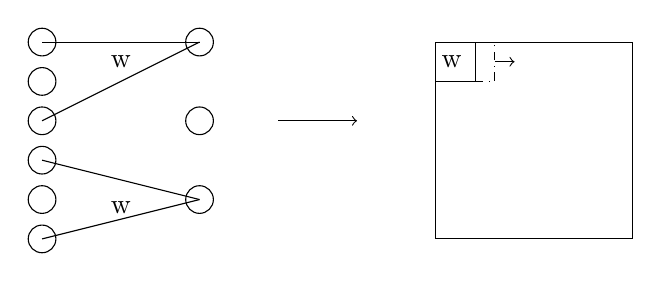
\begin{tikzpicture}
  \draw (0,0.0) circle (5pt);
  \draw (0,0.5) circle (5pt);
  \draw (0,1.0) circle (5pt);
  \draw (0,1.5) circle (5pt);
  \draw (0,2.0) circle (5pt);
  \draw (0,2.5) circle (5pt);

  \draw (2,0.5) circle (5pt);
  \draw (2,1.5) circle (5pt);
  \draw (2,2.5) circle (5pt);

  \draw (0,0.0) -- (2,0.5);
  \draw (0,1.0) -- (2,0.5);
  \draw (0,1.5) -- (2,2.5);
  \draw (0,2.5) -- (2,2.5);

  \node at (1,2.25) {w};
  \node at (1,0.40) {w};

  \draw[->] (3, 1.5) -- (4, 1.5);

  \draw (5,0) -- (7.5,0) -- (7.5,2.5) -- (5,2.5) -- (5,0);
  \draw (5,2) -- (5.5,2) -- (5.5,2.5) -- (5,2.5) -- (5,2);
  \draw[dash dot] (5.5,2) -- (5.75,2) -- (5.75,2.5);
  \draw[->] (5.75, 2.25) -- (6, 2.25);
  \node at (5.2, 2.25) {w};
\end{tikzpicture}

\paragraph{Note:}
\begin{itemize}
\item Stride: hyperparameter
\item Channel: number of weight matrices in the previous layer
\item Average Pooling, Max pooling(non-differentiable, heuristics are used for back propagation)
\end{itemize}

\paragraph{Other CNN based neural networks}
\begin{itemize}
\item ResNet-50: \\
  Residual block($x + \sigma(w^Tx)$) with 50 layers (residual block on every layer)
\item VGG
\end{itemize}

\section{Recurrent Neural Networks}
\label{sec:recurr-neur-netw}

\paragraph{Eg:} Machine translation (any time series data) \\
Datapoint: sentence (collection of words)
Cannot use MLP as every datapoint has a different dimension \\

\paragraph{Problems:}
\begin{itemize}
\item different input lengths
\item temporal dependency
\end{itemize}

\paragraph{Note:}
\begin{itemize}
\item CNN: parameter sharing across space
\item RNN: parameter sharing across time
\end{itemize}

\begin{tikzpicture}
  \draw[->] (0,0) -- (0,1);
  \draw (0,1.25) circle (5pt);
  \draw[->] (0,1.5) -- (0,2.5);
\end{tikzpicture}

\paragraph{Notations:}
\begin{itemize}
\item $X$: a sentence
\item $x^{(i)}$: a sentence
\item $x_t^{(i)}$: a word (represented by a one-hot vector with length as the number of words in dictionary)
\item BPTT: Back propagation through time
\end{itemize}

\subsection{Problem: Vanishing gradient}
\label{sec:probl-vanish-grad}

Since the weight $(w)$ is same for all words(across time), the gradient can get close to zero (i.e., the past is forgotten) during backpropagation.

\subsection{LSTM}
\label{sec:lstm}

\textit{Date: 30/03/2023}

\noindent Selectively remembers things.

\noindent GRU: Gated recurrent unit

\noindent Blog: \url{https://colah.github.io/posts/2015-08-Understanding-LSTMs/}

\begin{align*}
\text{(\textit{forget gate})  }  f_t &= \sigma \left( W_f \left[ a_{t-1}, x_t \right] + b_f \right) \\
\text{(\textit{input gate})  }    i_t &= \sigma \left( W_i \left[ a_{t-1}, x_t \right] + b_i \right) \\
\text{(\textit{output gate})  }    o_t &= \sigma \left( W_o \left[ a_{t-1}, x_t \right] + b_o \right) \\
\text{(\textit{gate gate})  }    g_t &= \sigma \left( W_c \left[ a_{t-1}, x_t \right] + b_c \right) \\
  c_t &= f_t \odot c_{t-1} + i_t \odot g_t \\
  a_t &= o_t \odot \sigma (c_t)
\end{align*}

\subsubsection{Gated Recurrent Unit (GRU)}
\label{sec:gated-recurrent-unit}

\begin{align*}
  z_t &= \sigma \left( W_z \left[ a_{t-1}, x_t \right] \right) \\
  \tilde{a}_t &= \sigma \left( W \left[ a_{t-1}, x_t \right] \right) \\
  a_t &= (1 - z_t) \odot a_{t-1} + z_t \tilde{a_t}
\end{align*}

% \includegraphics{figures/lstm.svg}

\section{Classification and Regression Trees (CART)}
\label{sec:class-regr-trees}

\paragraph{Decision trees:}
\begin{itemize}
\item Non-parametric
\end{itemize}

\begin{figure}
  \centering
  \begin{minipage}{0.5\textwidth}
    \centering
    \def\svgwidth{\columnwidth}
    \subimport{figures}{decision_tree.pdf_tex}
    \caption{Tree splitting}
    \label{fig:decision_tree}
  \end{minipage}%
  \begin{minipage}{0.5\textwidth}
    \centering
    \def\svgwidth{\columnwidth}
    \subimport{figures}{cart.pdf_tex}
    \caption{Data}
    \label{fig:cart}
  \end{minipage}
\end{figure}

\paragraph{Tree - Splitting}

\begin{align*}
\text{Let, } D_k &\subseteq D, \text{ } D_k = \left\{ (x, y) \in S: y = k \right\} \\
  D &= D_1 \cup D_2 \cup ... \cup D_c \\
  \text{Define } P_k &= \frac{|D_k|}{|D|} \text{  [ML estimate]}
\end{align*}

Given a split, Let $P_1, ..., P_k$ be the corresponding probability.
The split is a bad split if the distribution of a class over all the points is uniform. Hence we split the data inorder to maximize the KL-divergence between the class distribution and the uniform distribution (impure) \\

Maximize KL-divergence (i.e., decrease impurity)
\begin{align*}
  \max_p D_{KL}(p \parallel q) &= \sum_{i=1}^c p_i \log \frac{p_i}{q_i} \\
                        &= \sum \left( p_i \log p_i + p_i \log c \right) \\
  &= \sum p_i \log p_i + \log c\sum p_i
\end{align*}

Gini Index (another measure of impurity)
\begin{align*}
G(D_i) = \sum_{i=1}^c p_i(1 - p_i)
\end{align*}


\pagebreak
\section{Notes}
\label{sec:notes}

\begin{itemize}
\item Refer Prof. Sashtri's lectures for Statistial learning theory
\item Reference(youtube): Cornell CS4780
\item Convolution $\rightarrow$ flip the matrix then correlate (search convolution vs correlation)
  
\item Finding $P_{y|x}$: discriminative
\item Finding $P_x, P_{x|y}, P_{xy}$: generative + sampling
\item Distributional shift: test and training data have different distribution
\end{itemize}

\section{Homework}
\label{sec:homework}

\begin{itemize}
\item Work out \textbf{BPTT} manually for RNN and GRU
  
\item See that magnitude of gradient of loss with respect $w$ for RNN depends on eigenvalues of $w$ while in case of GRU it doesn't not.
\end{itemize}

\section{Hacks}
\label{sec:hacks}

\begin{itemize}
\item Run grid search over various random seeds
\end{itemize}

\end{document}
%%% Local Variables:
%%% mode: latex
%%% TeX-master: t
%%% End:
